%% V1.0
%% by Christopher Leith, udacl@cielsystems.com
\documentclass[10pt]{article}
\usepackage[a4paper, total={7in, 10in}]{geometry}

\usepackage[pdftex]{graphicx}    
\usepackage{cite}

%% For code snippets
\usepackage{listings}
\usepackage{color}

\definecolor{dkgreen}{rgb}{0,0.6,0}
\definecolor{gray}{rgb}{0.5,0.5,0.5}
\definecolor{mauve}{rgb}{0.58,0,0.82}

\lstset{
  frame=tb,
  language=C,
  aboveskip=3mm,
  belowskip=3mm,
  showstringspaces=false,
  columns=flexible,
  basicstyle={\small\ttfamily},
  numbers=none,
  numberstyle=\tiny\color{gray},
  keywordstyle=\color{blue},
  commentstyle=\color{dkgreen},
  stringstyle=\color{mauve},
  breaklines=true,
  breakatwhitespace=true,
  tabsize=3
}

\begin{document}

\title{Deep RL Learning - Deep Reinforcement learning for robots}
\author{Christopher Leith}
\maketitle

\label{sec:Introduction}
\section{Introduction}

In this project we demonstrate Deep Reinforcement Learning (RL) using the Q learning algorithm (DQN). 
In a simulated robotic arm in the ROS/Gazebo environment we create a DQN agent and  define reward 
strategies that enable the robotic arm system to learn how move its joints to achieve the task of touching 
a target object in the environment. There are 2 distinct sub tasks:

\begin{itemize}
 \item Task1 -
 Touch the target with any part of the arm with 90\% success rate.
 \item Task2 - 
 Touch the target with only the gripper base of the arm with 80\% success rate.
\end{itemize}

\section{Reward Strategies}
There are 3 categories of reward and penalties used to train the system. The code for implementing
these rewards are in ArmPlugin.cpp and excerpted below.

\subsection{Collision Rewards}
Whenever the simulation environment detects a collision of any objects it calls the callback function
onCollisionMsg(), excepted below. This function uses the argments supplied by ROS to determine which objects
collided. In particular we check if the target item was hit and, in the case for Task2, if also the gripper base
was hit. If so the primary goal of the robot has been achieved and the REWARD\_WIN rward is issued and the episode
is ended. If some other collision invoked the callback, such as the arm collioding with itself or the ground
the the negative REWARD\_LOSS is issued and again the episode is ended.
 
\begin{lstlisting}
void ArmPlugin::onCollisionMsg(ConstContactsPtr &contacts){
    ... // Loop code removed.
    const bool didSomethingHitTarget = 
        (strcmp(contacts->contact(i).collision1().c_str(), COLLISION_ITEM) == 0);
    const bool didGripperHit =
        (strcmp(contacts->contact(i).collision2().c_str(), COLLISION_POINT) == 0);

    if (didSomethingHitTarget && didGripperHit) // Remove && didGripperHit to enable Task1
    {
      rewardHistory = REWARD_WIN;
      newReward  = true;
      endEpisode = true;
      return;
    } else { // There was some other collision
      rewardHistory = REWARD_LOSS;
      newReward  = true;
      endEpisode = true;
    }
    ...
}
\end{lstlisting}

The code for ground contact is handled in ArmPlugin::OnUpdate(), excerpted below.

\begin{lstlisting}
void ArmPlugin::OnUpdate(const common::UpdateInfo& updateInfo){
    ... // Code removed
    const bool didHitGround = ( gripBBox.min.z <= groundContact || gripBBox.max.z <= groundContact );
    if (didHitGround)
    {
        if(DEBUG){printf("GROUND CONTACT, EOE\n");}
        rewardHistory = REWARD_LOSS;
        newReward     = true;
        endEpisode    = true;
    }
    ...
}
\end{lstlisting}


\subsection{Interim Rewards}
The interim rewards are rewards issued for each frame of an episode. The primary training object of this award
is to teach the robot to make progress towards the target. There were 2 options for for managing joint actions, 
either velocity control or position control. Although velocity control would provide more realistic physics
and pleasing visuals position control seemed far simpler to implement and so that was chosen for this implementation.

The code uses a time averaged progress to the target (avgGoalDelta) and uses that value to  determine whether progress is being made. 
towards the target. Larger values generate larger rewards. Additonally a constant 'lingerPunishment' is subtracted from the reward
to discourage little or no movement. 
These values were very much discovered by trial and error in coordination with the values of REWARD\_WIN and REWRD\_LOSS.
\begin{lstlisting}
void ArmPlugin::OnUpdate(const common::UpdateInfo& updateInfo){
    ... // Code removed
    const bool didHitGround = ( gripBBox.min.z <= groundContact || gripBBox.max.z <= groundContact );
    ...

    // Issue an interim reward based on the distance to the object
    if(!didHitGround)
    {
      const float distGoal = BoxDistance(gripBBox, propBBox); // compute the reward from distance to the goal
      if(DEBUG){printf("distance('%s', '%s') = %f\n", gripper->GetName().c_str(), prop->model->GetName().c_str(), distGoal);}

      if( episodeFrames > 1 )
      {
        const float distDelta  = lastGoalDistance - distGoal;
        const float movingAvgRC  = 0.4f;
        const float progressRewardFactor  = 4.0f;
        const float lingerPushisment  = 0.25f;

        // compute the smoothed moving average of the delta of the distance to the goal
        avgGoalDelta = (avgGoalDelta * movingAvgRC) + (distDelta*(1.0f - movingAvgRC));
        rewardHistory = avgGoalDelta * progressRewardFactor - lingerPushisment;
        newReward     = true;
      }

      lastGoalDistance = distGoal;
    }
    ...
}
\end{lstlisting}

\subsection{Timeout Reward}
In the case that the robot does not hit the target (or anything else) within 200 simulation frames, a negative reward is issued and 
the episode is ended.

\begin{lstlisting}
void ArmPlugin::OnUpdate(const common::UpdateInfo& updateInfo){
    ... // Code removed
    // episode timeout
    if( maxEpisodeLength > 0 && episodeFrames > maxEpisodeLength )
    {
        printf("ArmPlugin - triggering EOE, episode has exceeded %i frames\n", maxEpisodeLength);
        rewardHistory = REWARD_LOSS;
        newReward     = true;
        endEpisode    = true;
    }
    ...
}
\end{lstlisting}
 
 
\section{Hyperparameters}
The following hyperparameters were altered from the project template. 

\begin{lstlisting}
#define REWARD_WIN  20.0f
#define REWARD_LOSS -20.0f
\end{lstlisting}
The most important reward values were chosen empirically through trial an error. Although the absolute magnitudes are arbitrary
their relative values to each other and to the values used for interim rewards is critical.

\begin{lstlisting}
#define ALLOW_RANDOM true
#define EPS_DECAY 100
\end{lstlisting}
With ALLOW\_RANDOM permitting non-optimal action paths in the delevolping policy, the DQN can explore new paths through the state
space that could converge on a better policy. However the default EPS\_DECAY of 200 seemed to shut done this exploration to quickly
so a lower value was tried that seemed to allow continued improvement.

\begin{lstlisting}
#define INPUT_WIDTH   64
#define INPUT_HEIGHT  64
\end{lstlisting}
A smaller state space reduces processing and likely speeds convergence.
\begin{lstlisting}
#define OPTIMIZER "RMSprop"
\end{lstlisting}
RMSProp optimizer was chosen after Adam optimizer seemed to not work. In retrospect either may have worked after the other
parameters were tuned, but this was not tested.

\begin{lstlisting}
#define LEARNING_RATE 0.05f // Task1=0.01f Task2=0.05
\end{lstlisting}
A wide variety of learning rates were tested. The published results used the values as described in the comment, although in retrospect the tasks
most likely could have used either value but the successful runs were found most quickly using these emprically selected values. 

\begin{lstlisting}
#define BATCH_SIZE 64
#define USE_LSTM true
#define LSTM_SIZE 256
\end{lstlisting}
The batch size value did not seem to make much difference but may make GPU utilization more or less efficient. The LSTM memory was used
to keep a pool of previous states available for replay.


\section{Results}
Both tasks met the specified accuracy targets. The number of episodes to do so, however seemed to vary considerably.
The best recorded runs are shown in the figures below.

\subsection{Results - Task1}
Task1 was able to achieve 93\% accuracy by the 100th episode as seen in Fig ~\ref{fig:Task1Fast} 
and 96\% accuracy by the 221st episode as seen in Fig ~\ref{fig:Task1Good} 

\begin{figure}[p]
      \centering
      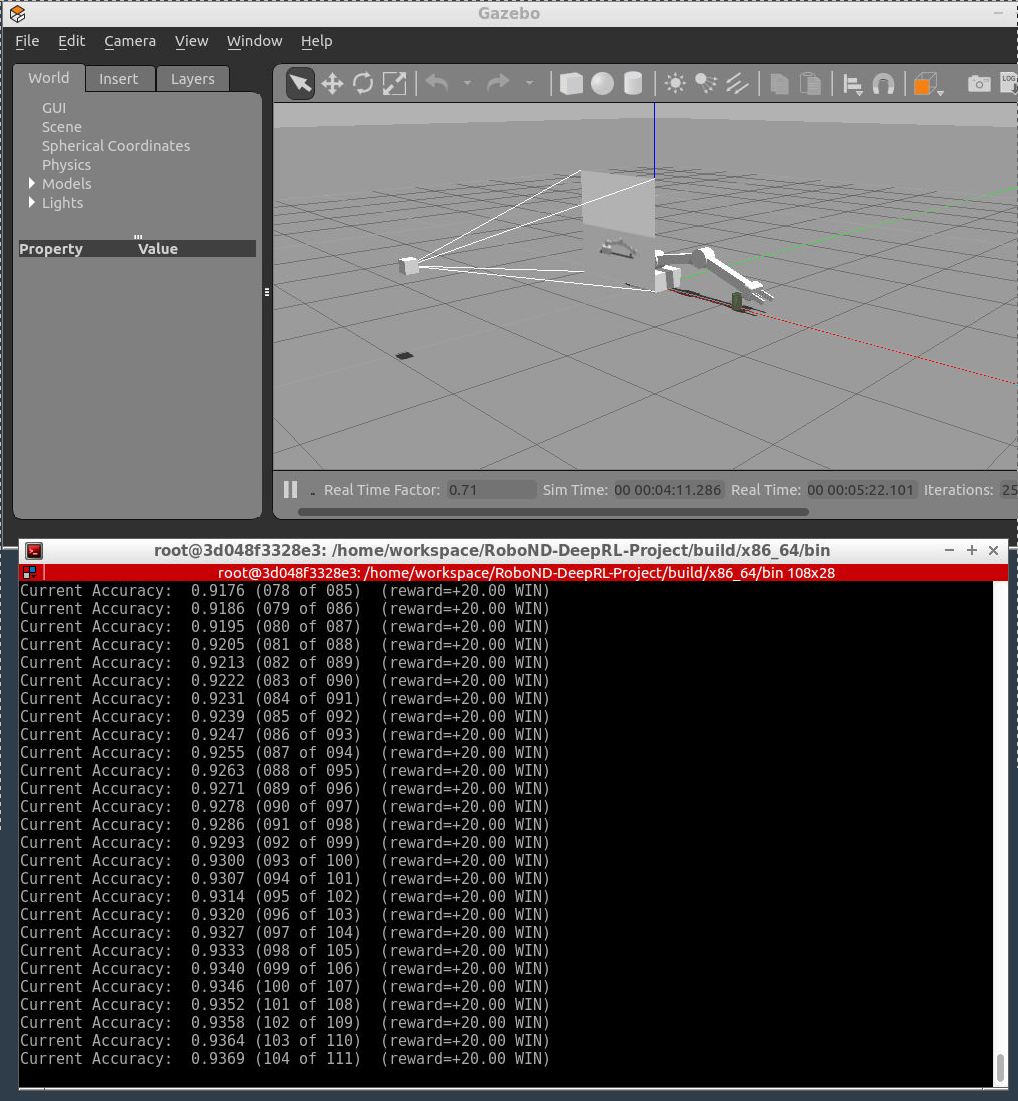
\includegraphics[width=\linewidth]{Assets/Task1_90at100_2019-03-05_08-45-06.png}
      \caption{Task1 Fast}
      \label{fig:Task1Fast}
\end{figure}

\begin{figure}[p]
      \centering
      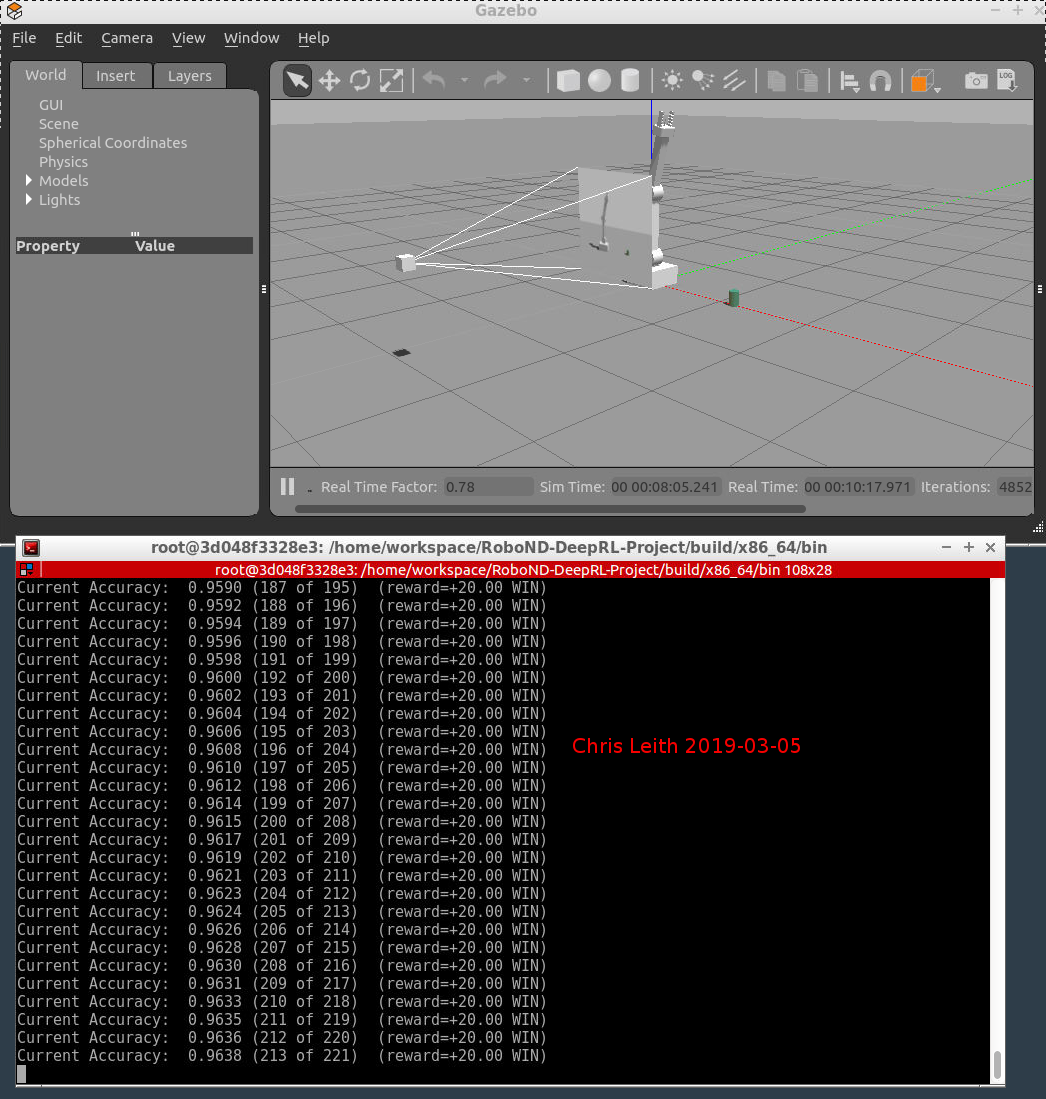
\includegraphics[width=\linewidth]{Assets/Task1_96at236_2019-03-05_08-45-06.png}
      \caption{Task1 Good}
      \label{fig:Task1Good}
\end{figure}

\subsection{Results - Task2}
Task2 was able to achieve 92\% accuracy by the 100th episode as seen in Fig ~\ref{fig:Task2Fast} 
and 95\% accuracy by the 211st episode as seen in Fig ~\ref{fig:Task2Good} 

\begin{figure}[p]
      \centering
      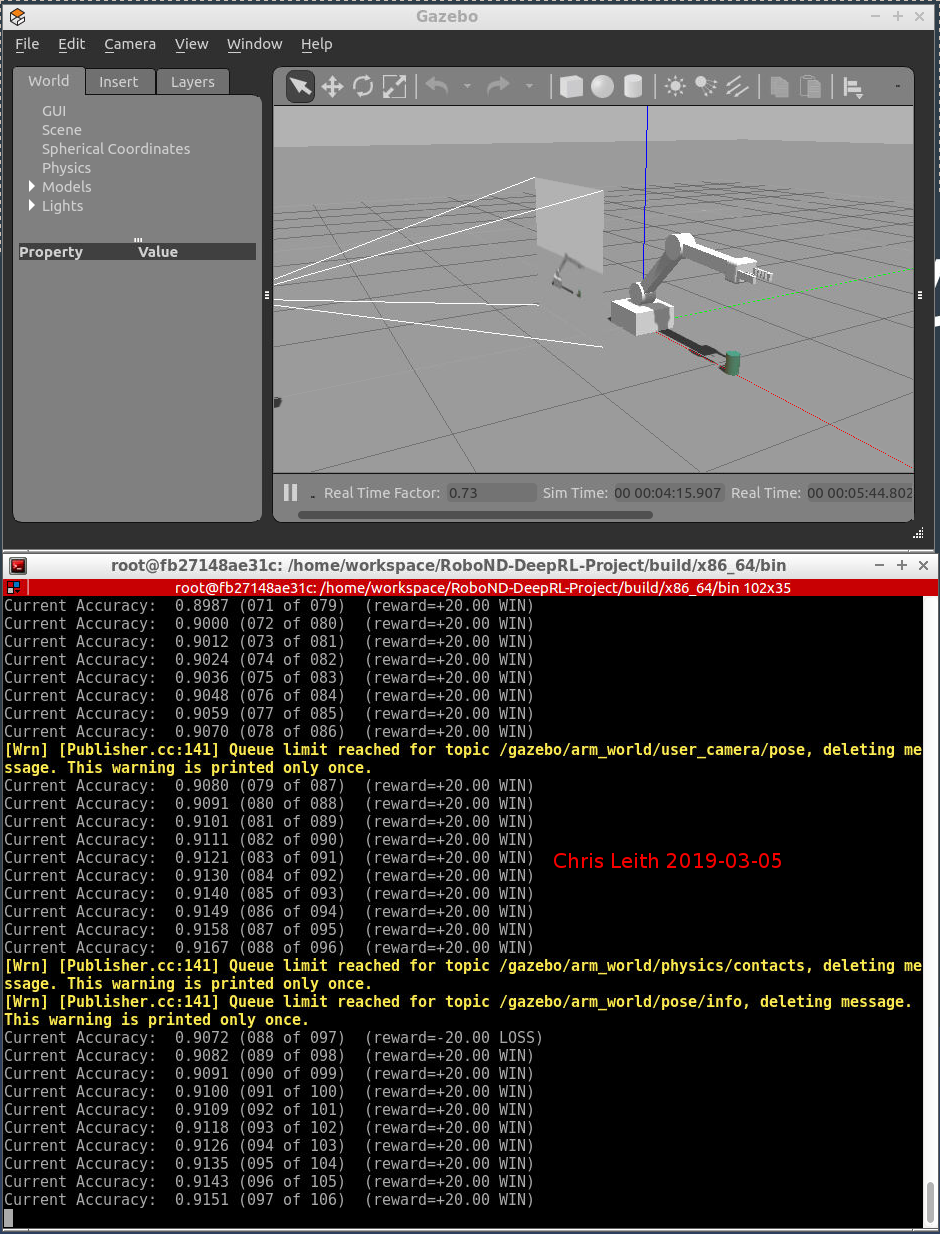
\includegraphics[width=\linewidth]{Assets/Task2_92at100_Learn0p05_2019-03-05_11-59-20.png}
      \caption{Task2 Fast}
      \label{fig:Task2Fast}
\end{figure}

\begin{figure}[p]
      \centering
      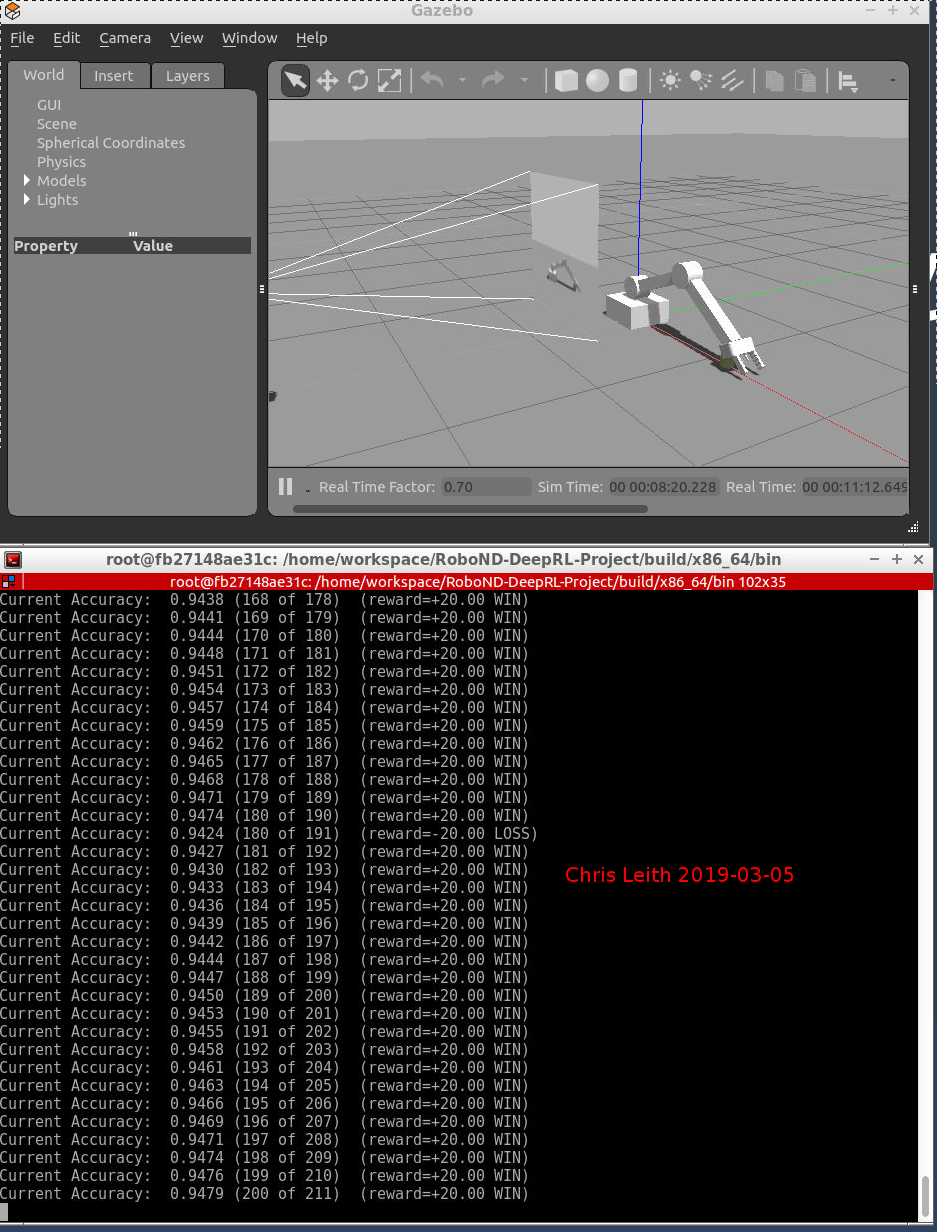
\includegraphics[width=\linewidth]{Assets/Task2_94at200_Learn0p05_2019-03-05_12-04-49.png}
      \caption{Task2 Good}
      \label{fig:Task2Good}
\end{figure}

\section{Discussion}
As always with hyperparameter tuning work proceeds in a haphazard manner and the success of changing parameters is very much path dependent. In the end a good result was achieved and the speed of convergence was most improved, it seemed, by including a interim penalty for failure to progress towards the
target. Without that penalty the arm frequently seemed to get "stuck" and timeout. This made the number of required episodes greater and the duration of each episode longer, which in turn made the tuning trials very timme consuming.
It was also observed that the same code converged differently on different runs making tuning frustrating. A good solution for this would be to control the random seed for the system so that parameter changes could be more reliably evaluated.    

\section{Conclusion / Future work}
This was another fun project. The theory in the lessons were quite intimidating but the project template provided a very gentle introduction to application of RL in robotics. And the use of ROS/Gazebo makes future experimentation more fun and approachable. With in this project itself it would be fun to go back and experiment with tuning with a generally working system. 

\end{document}